\section{Modello Analitico}
In questa sezione viene mostrata la metodologia utilizzata per la stima statistiche.
Nel modello analitico le statistiche si basano sui valori medi delle variabili
aleatorie $S$, $N$ e $X$, corrispondenti rispettivamente al tempo di risposta,
popolazione e throughput.

Per il calcolo delle metriche locali e globali, è stato inoltre necessario
ottenere la distribuzione stazionaria dello stato del cloudlet, in modo tale da
poter stabilire lo stato di tutto il sistema in condizioni di stazionarietà, e a
tale scopo, si è modellato il cloudlet come una catena di markov.
%
\subsection{Calcolo della distribuzione stazionaria}
Il generico stato della catena di markov è rappresentato da una coppia di interi
($n_1, n_2$) che indicano la quantità di job della relativa classe presenti nel
cloudlet.  

La frequenza di transizione da uno stato all'altro è regolata dai tassi di
arrivo $\lambda_1$ e $\lambda_2$ e di completamento $\mu_1$ e $\mu_2$.

La catena rispetta i vincoli imposti relativi alla somma delle variabili
(figura~\ref{ctmc})
\begin{figure}[!h]
\centering
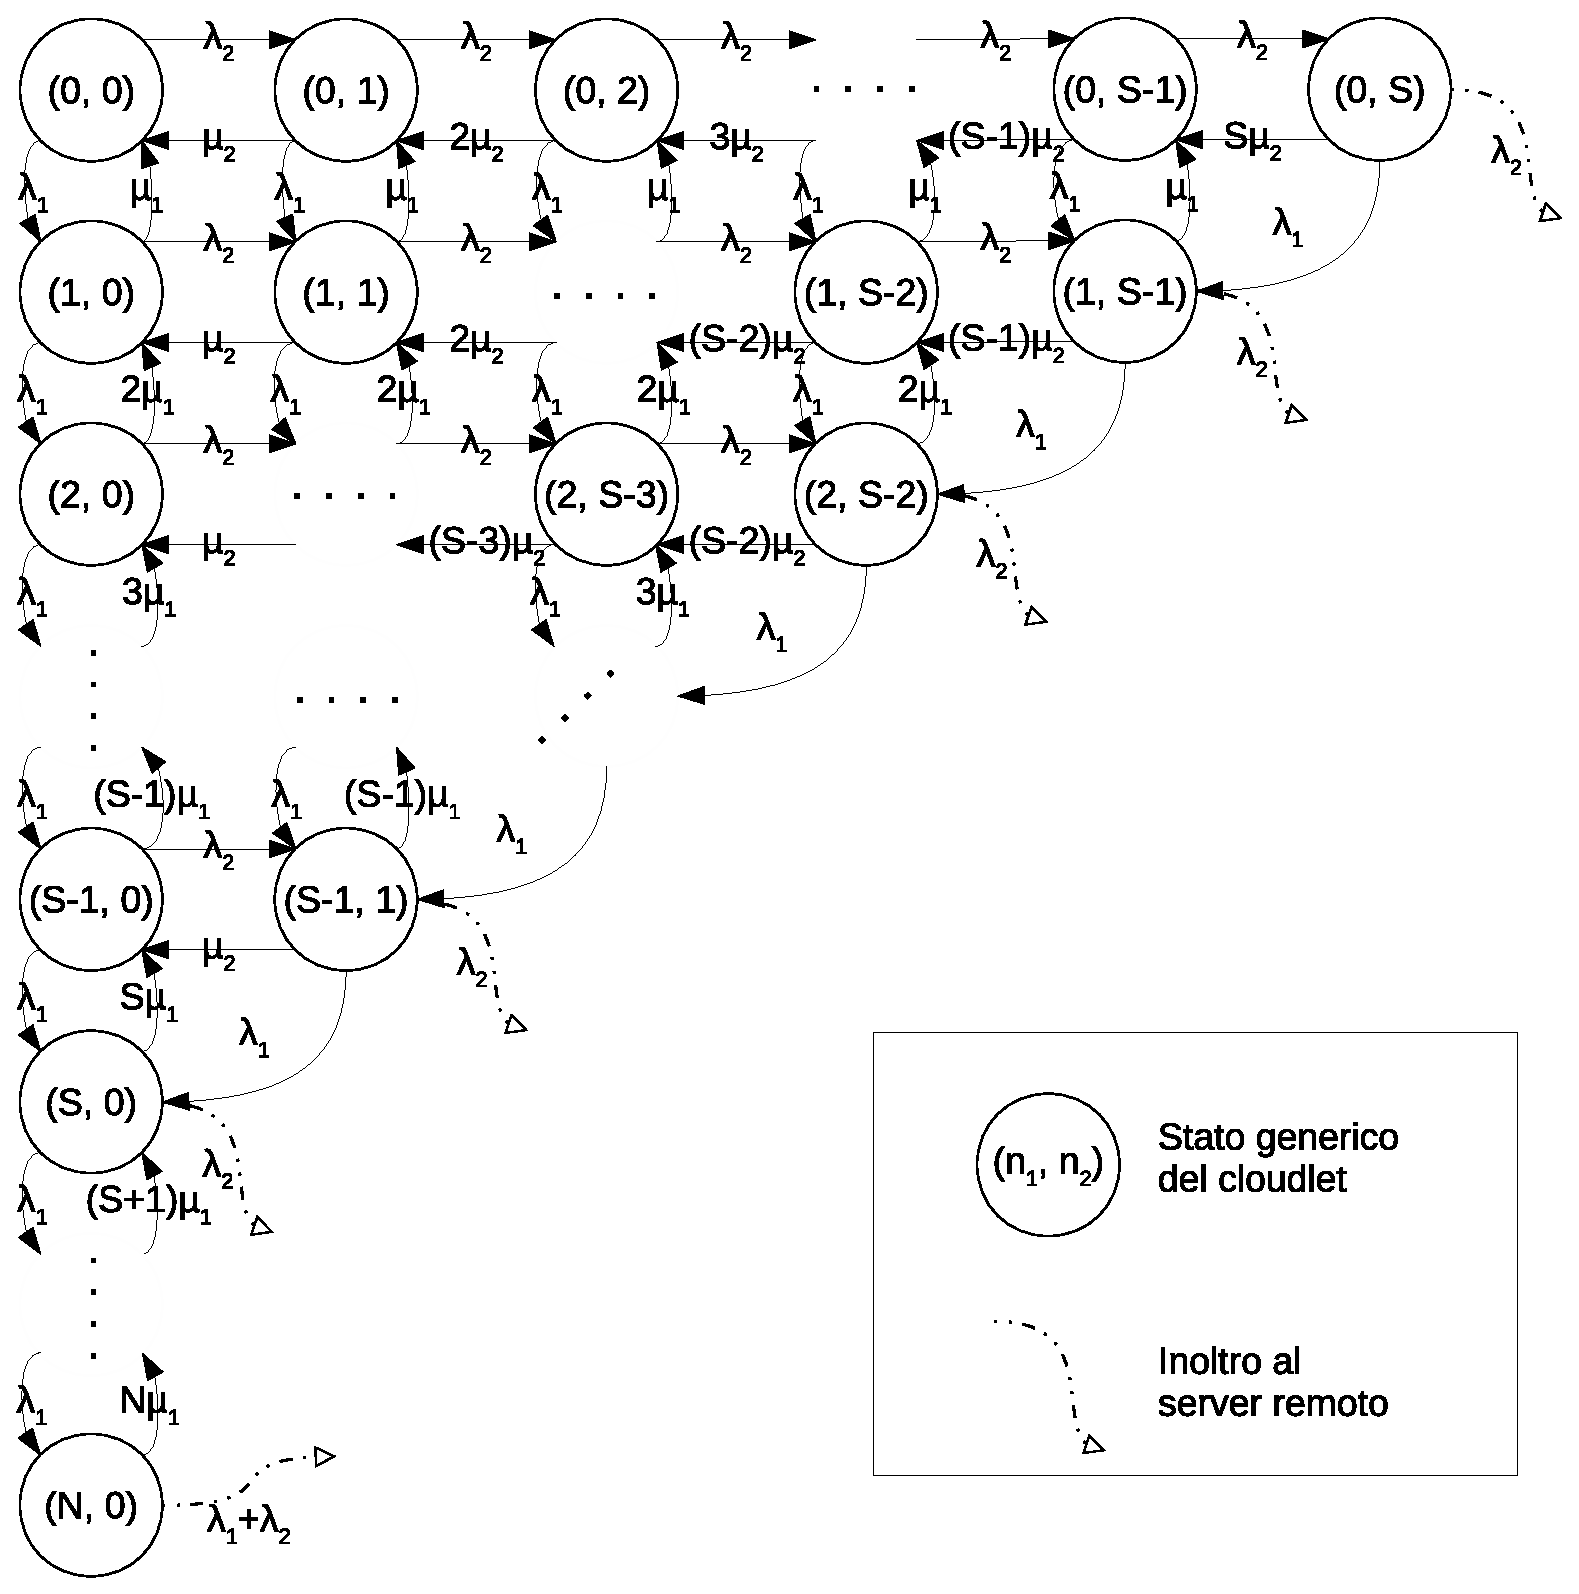
\includegraphics[width=0.7\textwidth]{figures/ctmc}
\caption{CTMC cloudlet}
\label{ctmc}
\end{figure}
